\section{Configuration Space Restrictions}
It is important to understand how the restrictions to the configuration space by~\eqref{eqn:departure_delay_model_discretization} influence the solution quality.
Therefore we solve~\eqref{eqn:departure_delay_model} with a constraint programming solver~\cite{numberjack} for various delay discretizations and upper bounds as well as for the continuous problem.
As problem instances we used most of the connected components of the conflict graph for $D_\text{max}=18$ minutes with up to $N_f=50$ flights and $N_c=104$ conflicts.
\begin{figure}[htpb]
    \centering
    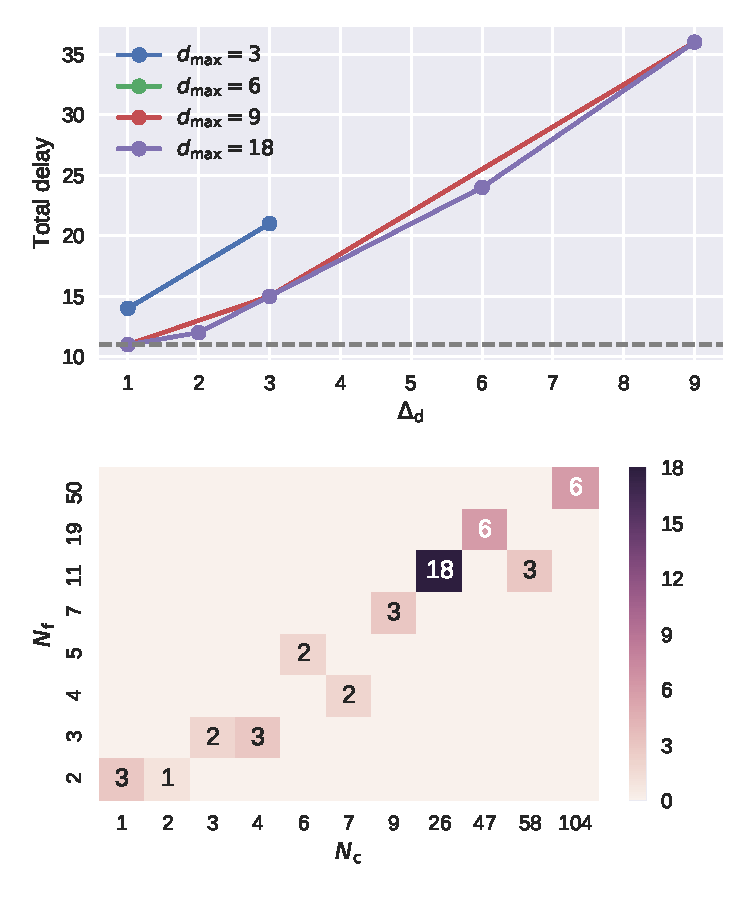
\includegraphics[width=0.45\textwidth]{./pics/delay_only_cp_results.pdf}
    \caption{Top: Total delay of constraint programming solutions for a problem instance with $N_f=19$ flights and $N_c=47$ conflicts for various discretization parameters.
    Bottom: Minimum $d_\text{max}$ which yield optimal solution in continuous problem for various problem instances. For all problem instances we used $D_\text{max}=18$ minutes.}
\label{fig:delay_only_cp_results}
\end{figure}

In figure~\ref{fig:delay_only_cp_results} one can see the results for a problem instance extracted from a connected component of the conflict graph with $N_f=19$ flights and $N_c=47$ conflicts.
With the exception of the small maximum delay $d_\text{max} = 3$ min, the total delay of the solutions is nearly independent of the maximum delay.
Moreover it is monotonically increasing with the coarseness of the discretization.
Since the original data is discretized in time in units of $1$ minute, $\Delta_t=1$ yield the same result as a continuous variable with the same upper bound.
Obviously the total delay for the continuous solution decreases monotonically with $d_\text{max}$.
Above a certain value $d^0_\text{max}$ the total delay stays the same.
With one exception, we found that for all the investigated problem instances $d^0_\text{max}\leq6$ minutes (see figure~\ref{fig:delay_only_cp_results}).
Therefore we conclude, that a moderate maximum delay is sufficient even for larger problem instances.
On the other hand, the delay discretization should be as fine as possible to obtain a high quality solutions.

